\documentclass[a4paper,fleqn]{cas-dc}

% If the frontmatter runs over more than one page, use the longmktitle option.
%\documentclass[a4paper,fleqn,longmktitle]{cas-dc}

% Neurocomputing: numbered citations in square brackets, in order of appearance.
\usepackage[numbers,sort&compress]{natbib}

\usepackage{amsmath,amssymb}
\usepackage{graphicx}
\usepackage{booktabs}
\usepackage{array}
\usepackage{xcolor}
\hypersetup{linkcolor=blue,citecolor=blue,urlcolor=blue}

\newcommand{\todo}[1]{\textcolor{red}{[TODO: #1]}}
% cas-common already defines L/R/C column types; P is our ragged-right paragraph column.
\newcolumntype{P}[1]{>{\raggedright\arraybackslash}p{#1}}
\setlength{\emergencystretch}{1.5em}

% ---- Author info: edit here only ------------------------------------
\newcommand{\AuthorName}{Younghoon Kang}
\newcommand{\AuthorShort}{Y. Kang}
\newcommand{\AuthorEmail}{kangyh61@seoultech.ac.kr}
\newcommand{\AuthorOrg}{Seoul National University of Science and Technology}
\newcommand{\AuthorCity}{Seoul}
\newcommand{\AuthorCountry}{Republic of Korea}
% ---------------------------------------------------------------------

\begin{document}
\let\WriteBookmarks\relax
\def\floatpagepagefraction{1}
\def\textpagefraction{.001}

\shorttitle{Order-preserving temporal pooling for CPU-efficient video CIL}
\shortauthors{\AuthorShort}

\title [mode = title]{OPTP: CPU-efficient Incremental Video Recognition  with Order-preserving Temporal Pooling}

\author[1]{\AuthorName}
\cormark[1]
% \ead prints its argument verbatim, so the macro must be expanded first
\expandafter\ead\expandafter{\AuthorEmail}
\credit{Conceptualization, Methodology, Software, Validation, Formal analysis, Investigation, Data curation, Visualization, Writing -- original draft, Writing -- review \& editing}
\affiliation[1]{organization={\AuthorOrg},
            city={\AuthorCity},
            country={\AuthorCountry}}

\cortext[1]{Corresponding author}

\begin{abstract}
Deployed vision systems must recognize new classes after shipping without
forgetting old ones, and on constrained hardware this rules out
backpropagation entirely: fine-tuning a small recurrent baseline costs
270\,s per session in our own tests, against 42.4\,ms for a closed-form
update, a $6{,}400\times$ gap. Video adds a difficulty that
frozen-backbone, gradient-free methods have not addressed: some action
classes are defined only by the order motion occurs in, and mean pooling,
the standard way to summarize a clip, is invariant to that order by
construction. We introduce order-preserving temporal pooling, which splits
a window into $k$ contiguous segments and concatenates their means so that
early-then-late and late-then-early occupy different coordinates instead
of collapsing to the same vector. Paired with a closed-form covariance
head (FeCAM), the resulting pipeline uses zero learnable parameters and
zero gradient steps at any point after the backbone is frozen. On UCF101
under the TCD protocol, it ranks second behind only a method that trains a
temporal encoder with backpropagation, despite using zero exemplars and
zero gradient steps itself, and is the only method in that comparison
whose last-session accuracy is exactly invariant to how finely incremental
sessions are grouped. The pooling gain over mean pooling holds at $3.6\times$ the class
count on SSv2's standard 174-class split, and all nine pooling-and-head
combinations tested run comfortably within a 10\,fps CPU budget.
\end{abstract}

\begin{highlights}
\item Order-preserving temporal pooling for video class-incremental learning.
\item Zero learnable parameters and zero gradient steps after the backbone.
\item Ranks second on UCF101 (TCD protocol) with no exemplars or backprop.
\item Last-session accuracy is exactly invariant to session grouping.
\item Head update takes 42.4\,ms on CPU versus 270\,s for a GRU baseline.
\end{highlights}

\begin{keywords}
class-incremental learning \sep video recognition \sep temporal pooling
\sep exemplar-free \sep closed-form classifier \sep edge computing
\end{keywords}

\maketitle



% =====================================================================
\section{Introduction}
\label{sec:intro}
% =====================================================================

Deployed vision systems are rarely trained once and left alone. A household
robot, a pair of smart glasses, or an IoT camera is expected to recognize new
object or action categories after it has already shipped, and it must do so
without forgetting what it already knew. Class-incremental learning (CIL)
formalizes this requirement: given a sequence of class sets that arrive over
time, a model must learn each new set while retaining accuracy on all
previously seen classes, typically without revisiting their original data.
The alternative (collecting all data seen so far and retraining from
scratch) becomes prohibitively expensive as the number of classes grows,
and it is frequently not an option at all, since edge devices cannot always
reach a server and may not be permitted to retain raw user data. Naive
retraining is not merely inconvenient; the cost gap is measured in orders of
magnitude. In our own stack, fitting a closed-form classification head takes
42.4\,ms, while fine-tuning a small recurrent baseline with backpropagation
on the same data takes 270\,s, roughly $6{,}400\times$ more (see
Section~\ref{sec:experiments}). If registering one new class stalls a
real-time pipeline for minutes, the deployment scenario collapses regardless
of accuracy.

Video class-incremental learning inherits every difficulty of image CIL and
adds one that a single frame cannot resolve. Some categories fail a simple
test: freeze the video at any one frame, and nothing in it says which
class you are looking at. In Something-Something V2 (SSv2), \emph{pulling
something from left to right} and \emph{pulling something from right to
left} share the same objects, the same background, even the same
individual frames as a set: only the order they play in differs. A model
that pools
frame features by simple averaging cannot distinguish the two, because mean
pooling is invariant to permutation of its inputs and therefore destroys the
one signal that separates the classes (we verify this collapse directly in
Section~\ref{sec:method-pooling}). Video CIL is thus the conjunction of two
open problems: incremental learning under storage and compute constraints,
and temporal modeling under a closed-form, gradient-free budget.

CPU-only operation is not a minor implementation detail; it is the binding
constraint that most prior work quietly assumes away. The video-CIL
literature we survey in Section~\ref{sec:related} reports strong accuracy
numbers but is uniformly silent on wall-clock training time or CPU
throughput, because every one of those methods fine-tunes its backbone (or a
substantial module on top of it) with backpropagation across every
incremental session. That assumption is reasonable for a benchmark run on a
GPU cluster; it is not reasonable for a robot, a headset, or a camera that
must register a new class in real time on its own processor, on battery, and
without network access.

Existing approaches leave this intersection largely unexplored precisely
because they optimize a different axis. The frozen-backbone,
rehearsal-free line of image-CIL work has already shown that a good frozen
representation plus a lightweight statistical head can outperform far more
elaborate learned classifiers, but that evidence comes entirely from static
image benchmarks with no temporal axis to preserve. Video-CIL methods that
do model time do so by training the backbone or a temporal module on the
target domain with full backpropagation, which reintroduces the GPU
dependency we are trying to remove. Edge-CIL surveys acknowledge the
computational constraint explicitly, but define ``edge'' almost entirely in
terms of memory budget and defer the compute and latency axes to future
work. No existing comparison table places video, CPU-only operation, and a
real-time throughput budget on the same axis at once; that intersection is
the gap this paper addresses.

Our approach keeps a frozen CLIP backbone and a closed-form covariance-based
head (FeCAM~\cite{goswami2023fecam}) exactly as prior frozen-representation work does, and adds a
single new ingredient: a pooling function that preserves the order of the
frames it summarizes instead of averaging them away. The window is split
into $k$ contiguous temporal segments, each segment is reduced to its own
mean, and the segment means are concatenated so that each carries a fixed,
distinguishable position in the output vector. The representation of
\emph{early-then-late} and \emph{late-then-early} can no longer coincide,
because they now occupy different coordinates rather than being averaged
into the same one. We also tried the standard fix for boundary artifacts in convolutional and
spectral pooling: widening the segments so that neighbors overlap. Here it
backfires: accuracy degrades monotonically instead of improving. We unpack
this negative result in Section~\ref{sec:method-pooling}, since it
clarifies why the segmentation itself works and overlap does not. Both the
pooling function and the FeCAM head require zero gradient steps at
enrollment time, so the ``no training after deployment'' property of the
frozen-backbone track is preserved while its main limitation, an inability
to represent order, is directly addressed.


% =====================================================================
\section{Related Works}
\label{sec:related}
% =====================================================================

\subsection{CIL for Video Recognition}

\textbf{Video CIL benchmarks.} vCLIMB~\cite{villa2022vclimb} established UCF101,
ActivityNet, and Kinetics as a standard video-CIL benchmark suite and
introduced the convention of accounting for replay memory in \emph{frame
count} rather than instance count, an early acknowledgment that memory
means something different for video than for images. Its TSN+ResNet-34
baseline reports 81.0 on UCF101 and 32.0 on Kinetics with iCaRL-style~\cite{rebuffi2017icarl}
rehearsal. We evaluate on UCF101 as well (Section~\ref{sec:experiments}),
but under the TCD lineage's protocol below rather than vCLIMB's own split,
since that is the protocol our closest points of comparison use.

\textbf{SSv2 as a CIL benchmark.} A separate lineage uses Something-Something
V2 directly as the class-incremental testbed, which is the branch most
directly relevant to this work since it is the same dataset we evaluate on.
Table~\ref{tab:tcd-lineage} summarizes five papers in this lineage, verified
against their original PDFs rather than secondary citations.

\begin{table*}[pos=!t]
\centering
\caption{SSv2 class-incremental methods. TCD, STSP, and CSTA report on the
identical 174-class split (84 base $+$ [$10{\times}9$] or [$5{\times}18$]
incremental); CIVC predates that split and uses its own 40-class subset, so
its number is not directly comparable and is included for its independent
methodological argument (see text).}
\label{tab:tcd-lineage}
\small
\renewcommand{\arraystretch}{1.15}
\begin{tabular}{@{}lP{1.6cm}P{2.1cm}P{2.3cm}l@{}}
\toprule
Method & Venue & Exemplar & Backbone & SSv2 ($10{\times}9$/$5{\times}18$) \\
\midrule
TCD~\cite{park2021tcd} & ICCV'21 & 20/class & ResNet-50+TSM & 35.78 / 29.60 \\
CIVC~\cite{zhao2021civc}$^\dagger$ & ACM MM'21 & 5/class + key-frame & TSM-ResNet50 & 46.30 (own 40-cls split) \\
STSP~\cite{cheng2024stsp} & ECCV'24 & 0 (exemplar-free) & ResNet-50+TSM & \textbf{69.68} / \textbf{70.87} \\
CSTA~\cite{chen2025csta} & IEEE T-CSVT'25 & 5/class (FT)$^\ddagger$ & TimeSformer & 41.26 / -- \\
ESSENTIAL~\cite{lee2025essential} & ICCV'25 (HL) & sparse + prompt & frozen CLIP & 48.9 / 47.5 \\
\bottomrule
\end{tabular}
\end{table*}

\noindent\textit{Backbone abbreviations:} TCD/STSP use ResNet-50+TSM~\cite{lin2019tsm}
(fine-tuned throughout for TCD, adapted via null-space projection for
STSP); CIVC uses TSM-ResNet50 (trained via trajectory-guided distillation);
CSTA adds spatiotemporal adapters on TimeSformer~\cite{bertasius2021timesformer}; ESSENTIAL keeps CLIP
frozen and adds a learned temporal encoder on top. The full description of
each backbone's training regime is in the paragraph below the table.

$^\dagger$CIVC uses a different, earlier 40-class subset (20 base $+$ 20
incremental across 5 sessions) and is not directly comparable on the
accuracy column; its relevance is methodological, discussed below.
$^\ddagger$CSTA is described as exemplar-free in its title and abstract, but
its own implementation section states that a per-task fine-tuning stage
draws 5 real samples per class from previous tasks to construct a balanced
set, ``aligning with the definition in the TCD Benchmark,'' and this
fine-tuned classifier is what produces the headline numbers in
Table~\ref{tab:tcd-lineage} (verified directly against the CSTA PDF).

\textbf{A trained-representation track.} TCD, STSP, and CSTA all adapt their backbone to SSv2 with full
backpropagation (gradient updates and constraints for TCD and STSP, adapter
training for CSTA), so every feature these three methods report is a
representation that has been exposed to SSv2 motion during training.
ESSENTIAL is the only member of this lineage that keeps its visual encoder
(CLIP) entirely frozen, but it still trains a temporal encoder and a
memory-retrieval module on top of it with backpropagation; per its own
implementation details, this training uses 24 NVIDIA RTX 3090 GPUs (8 for
UCF101/ActivityNet) with 50 epochs of current-task training plus 30 epochs
of rehearsal training per task. All five methods therefore belong to a track
that trains its representation on the target domain; we belong to a track
that never does. We report our own numbers on this exact 174-class split in
Section~\ref{sec:experiments}. None of the five papers reports wall-clock training time
or CPU inference throughput, consistent with a literature that has not had
to justify itself on those axes because GPU access is assumed.

\textbf{CIVC's independent diagnosis.} CIVC~\cite{zhao2021civc}
deserves separate attention because it reaches a conclusion structurally
identical to ours from a different part of the pipeline. Rather than pooling
frame-level features before distillation, CIVC decomposes the fused
spatiotemporal feature using motion-trajectory information and distills the
decomposed representation; on its own 40-class SSv2 subset this raises
accuracy from a fused baseline of 40.79 to 45.87 with decomposition alone,
and to 46.30 with trajectory-guided decomposition. The paper motivates this
choice with the same example we use independently in
Section~\ref{sec:intro-example}: \emph{``the Something-Something V2 dataset
incorporates concepts of left and right, e.g., pulling something from left
to right and pulling\ldots''}: a left/right, order-sensitive pair that
naive pooling or fusion cannot distinguish. CIVC is exemplar-based (5
samples per video plus key-frame storage) and trains its TSM-ResNet50
backbone via distillation, so it sits in the same backprop-dependent track
as TCD/STSP/CSTA; what it shares with our work is not the mechanism but the
diagnosis: \emph{averaging or fusing temporal features destroys exactly the
information that SSv2-style classes depend on}, reached independently at a
different stage of the pipeline (knowledge distillation rather than
pooling).

\textbf{Our resolution.} Where prior work resolves this diagnosis by training a component to recover
temporal structure, we resolve it without training anything: mean pooling
is replaced by a fixed, order-preserving segment pooling function, and no
gradient is computed at any point after the backbone is frozen
(Section~\ref{sec:method-pooling}).

\subsection{CIL for CPU-only Edge Devices}

\textbf{Closed-form heads.} A streaming, closed-form line of work removes backpropagation from the
classifier itself. Streaming LDA (SLDA)~\cite{hayes2020slda} maintains a running mean
per class and a single shared covariance matrix, updated in closed form as
new data arrives: no gradient step, no replay buffer. FeCAM~\cite{goswami2023fecam}
extends the same shared-covariance idea with a sign-preserving Tukey
transform on the features and data-driven shrinkage of the covariance
estimate; we adopt FeCAM as our head and justify that choice directly in
Section~\ref{sec:method-fecam}.

\textbf{Edge-constrained CIL.} A separate body of work addresses edge constraints explicitly, but treats
compute and latency as an open question rather than a solved one. Zhou et
al.'s CIL survey~\cite{zhou2024cilsurvey} is the standard reference
maintained by the authors of PyCIL; it defines the edge setting almost
entirely in terms of \emph{memory} budget, explicitly states that dynamic
network architectures are unsuitable for edge deployment, and places the
compute and time axes in its Future Directions section rather than treating
them as already addressed. SparCL~\cite{wang2022sparcl} is a rare exception that
reports an actual on-phone CPU training measurement rather than an abstract
budget, which is closer to the empirical standard we hold ourselves to in
Section~\ref{sec:experiments}.

\textbf{Our approach.} Our approach takes the lightest baseline these two lines of work already
established (a frozen backbone with a closed-form covariance head) and
adds the smallest possible ingredient needed to make it viable for video:
an order-preserving pooling function with zero additional parameters and
zero additional gradient steps.


% =====================================================================
\section{Method}
\label{sec:method}
% =====================================================================

\subsection{Problem Formulation}
\label{sec:method-formulation}

\textbf{Setting.} We consider exemplar-free class-incremental learning. At session
$t = 1,\ldots,T$, a set of new classes $C_t$ arrives together with training
data for those classes only; once session $t$ ends, the raw data of
$C_1,\ldots,C_{t-1}$ is no longer available. Evaluation at session $t$ is a
$\left(\bigcup_{i \le t} |C_i|\right)$-way classification problem over every
class seen so far, with no task or session identifier provided at test time
(class-incremental, not task-incremental). We additionally require, as a
condition on the method rather than the benchmark: zero gradient
computations after deployment, CPU-only execution, and a per-frame budget of
100\,ms (i.e.\ a 10\,fps real-time target).

\textbf{Notation.} A video $v$ is uniformly sampled into 16 frames and
passed through a frozen encoder $f$, producing per-frame features
$W \in \mathbb{R}^{16 \times D}$. A pooling function
$\phi : \mathbb{R}^{16 \times D} \to \mathbb{R}^{D'}$ reduces this to a
single embedding $z = \phi(W)$, and a classification head scores $z$ against
the classes seen so far. Both $f$ and $\phi$ are fixed throughout: $f$ is
never fine-tuned, and $\phi$ has no learnable parameters at all.

\subsection{FeCAM}
\label{sec:method-fecam}

\textbf{A three-rung ladder.} We motivate the head as a three-rung ladder of increasing use of covariance
structure. \textbf{NCM} (nearest class mean) keeps only the per-class mean
and treats every feature direction as equally informative, so directions
along which a class varies a great deal and directions along which it barely
varies are weighted identically. \textbf{SLDA} multiplies by the inverse of
a single shared covariance matrix (the precision matrix) to compute a
Mahalanobis distance, which down-weights high-variance directions and
up-weights low-variance, high-signal directions: an explicit statement of
which axes actually discriminate between classes.
\textbf{FeCAM}~\cite{goswami2023fecam} builds on this with (A) a feature
preprocessing step, a sign-preserving Tukey transform
$\mathrm{sign}(x)|x|^{0.5}$ followed by $L_2$ normalization, and (B)
data-driven shrinkage of the covariance,
$\Sigma_s = \Sigma + \gamma_1 V_1 I + \gamma_2 V_2 (1-I)$, where $V_1$ and
$V_2$ are the average diagonal and off-diagonal (co)variance and
$\gamma_1=\gamma_2=1$ matches the many-shot CIL setting in the original
paper. Measured under the same protocol, accuracy rises monotonically
along this ladder (Section~\ref{sec:experiments}).

\textbf{Shared covariance.} We use the \emph{shared} covariance variant rather than FeCAM's main
per-class variant, and this is not an arbitrary simplification. The
original paper's primary method maintains one covariance matrix $\Sigma_y$
per class; the shared variant $\Sigma_{1:t}$ is presented as an explicit,
separately benchmarked, memory-efficient alternative. We adopt it because of
the memory structure we measure directly: filling all 256 class slots costs
only 4.2\,MB for the class means, while the two $D \times D$ covariance and
precision matrices dominate at 67\,MB ($D{=}2048$). A per-class covariance
would multiply that 67\,MB by the number of classes (3.2\,GB at 48 classes,
11.7\,GB at 174), which is incompatible with the CPU-only edge setting this
paper targets. Choosing the shared variant trades a small amount of
accuracy for a space complexity that is $O(1)$ in the number of classes
rather than growing with it, which is precisely the trade-off this work
needs.

\subsection{Order-Preserving Temporal Pooling}
\label{sec:method-pooling}

\textbf{Mean pooling destroys the temporal axis.}
\label{sec:intro-example}
Averaging frame features is invariant to the order of the frames being
averaged. In SSv2, ``pushing something from left to right'' and ``pushing
something from right to left'' involve the same object, the same
background, and (as a multiset) the same individual frames: the sequences
differ only in order, and mean pooling maps both to the identical vector.
TCD makes the same observation from a different angle, reporting that a
nearest-mean classifier underperforms a trained CNN specifically on SSv2
because ``na\"ive averaging of the features from all frames may not be
suitable.'' Our response addresses this by construction rather than by
training: we replace the pooling function, not the classifier.
Figure~\ref{fig:pooling-diagram} illustrates both the collapse and our fix
before we state either formally.

\begin{figure*}[width=\textwidth,pos=!t]
\centering
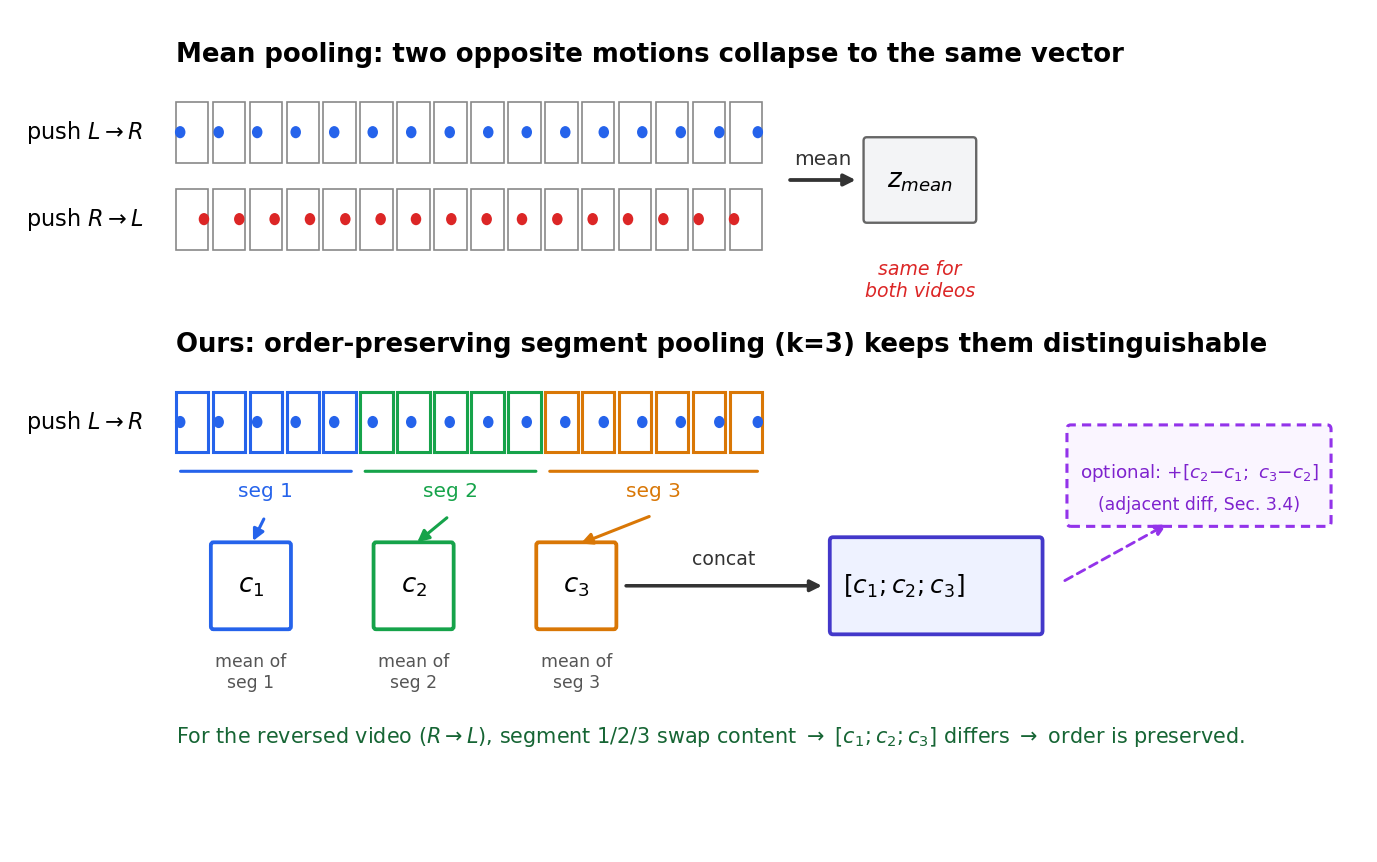
\includegraphics[width=\textwidth]{assets_pooling_diagram.png}
\caption{Top: mean pooling maps two opposite motions (left-to-right vs.\
right-to-left) to the identical vector $z_{\mathrm{mean}}$, since averaging
is invariant to frame order. Bottom: our order-preserving segment pooling
($k{=}3$) instead assigns each temporal segment its own fixed slot in the
output; concatenating $[c_1;c_2;c_3]$ preserves which content occurred
early versus late, so the two motions no longer coincide. The optional
adjacent-difference term (Section~\ref{sec:method-diff}) is shown as a separate,
dashed branch to emphasize that it is evaluated independently of the
segmentation itself.}
\label{fig:pooling-diagram}
\end{figure*}

\textbf{Scope.} Attaching a learned temporal encoder (e.g.\ a
transformer, as ESSENTIAL does) would recover order information, but it
requires backpropagation and therefore forfeits the premise of this paper.
We instead ask a narrower, closed-form question: \emph{how much of the
temporal information mean pooling discards can be recovered without
training anything at all?}

\textbf{Proposed pooling.} A window $W \in \mathbb{R}^{T \times D}$
($T{=}16$) is split into $k$ contiguous segments with boundary indices
\begin{equation}
b_i = \left\lfloor \frac{iT}{k} \right\rfloor, \quad i = 0,1,\ldots,k
\end{equation}
(when $T$ does not divide evenly by $k$, later segments absorb the extra
frames; for $T{=}16,\,k{=}3$ the segments are $5/5/6$ frames), and each
segment is reduced to its own mean,
\begin{equation}
c_i = \frac{1}{b_i - b_{i-1}} \sum_{t=b_{i-1}}^{b_i - 1} W_t \;\in\; \mathbb{R}^D,
\quad i = 1,\ldots,k .
\end{equation}
Segment-only pooling preserves order by concatenation:
\begin{equation}
\phi_{\mathrm{seg}}(W) = [c_1;\,c_2;\,\ldots;\,c_k] \in \mathbb{R}^{kD}
\;\Longrightarrow\; D'(k) = kD .
\end{equation}
An optional variant additionally concatenates the differences between
adjacent segments, treated as a separate mechanism and evaluated on its own
in Section~\ref{sec:method-diff}:
\begin{equation}
\begin{split}
\phi_{\mathrm{seg+diff}}(W) &= [c_1;\ldots;c_k;\; c_2{-}c_1;\ldots;c_k{-}c_{k-1}]\\
&\in \mathbb{R}^{(2k-1)D}
\;\Longrightarrow\; D'(k) = (2k-1)D ,
\end{split}
\end{equation}
since $k$ segments produce $k{-}1$ adjacent pairs. Both variants of $\phi$
have \emph{zero parameters, zero gradient steps, zero training}: each is a
fixed function of a $(16,512)$ array. With $D{=}512$ (CLIP B/32),
$\mathtt{chunks4}$ ($k{=}4$, segments only) gives $D'{=}2048$ and
$\mathtt{chunks3{+}adjdiff}$ ($k{=}3$, segments $+$ diff) gives $D'{=}2560$;
the remaining combinations and their measured accuracy are reported in
Section~\ref{sec:experiments}.

\textbf{Why it works.} Two controlled observations explain the
mechanism. \emph{First}, coarse order recovers most of the benefit: halving
the window into just two segments (``what it looked like in the first
half'' vs.\ ``the second half'') already recovers +7.00 percentage points,
78\% of the total gain over mean pooling: the crudest possible ordering
information does most of the work, which is the central intuition behind
using a closed-form pooling function at all rather than a learned one.
\emph{Second}, order-blind statistics do not help: appending the per-frame
standard deviation (\texttt{mean+std}), which is permutation-invariant and
therefore carries no order information despite doubling the output
dimension, buys only +1.04\,pp. Contrasted with the first observation, this
rules out dimensionality as the confound: the gain comes from restoring
order, not from adding coordinates.

\textbf{An inverted-U in segment count.} Increasing $k$ improves
temporal resolution but also grows the dimension $D'=kD$, and FeCAM must
estimate a $D' \times D'$ covariance from a limited number of samples per
class; once the dimension-to-sample ratio crosses a threshold, additional
segments cost more in estimation error than they gain in resolution.
Accuracy consequently traces an inverted U in $k$, peaking at 3--4 segments
at our data scale (Figure~\ref{fig:inverted-u}; full sweep in
Section~\ref{sec:experiments}). This temporal-resolution-versus-estimability
trade-off is an intrinsic property of the method, not a tuning artifact; we
would expect the optimal $k$ to grow with the number of samples available
per class, though we have not verified this.

\begin{figure}[pos=!htb]
\centering
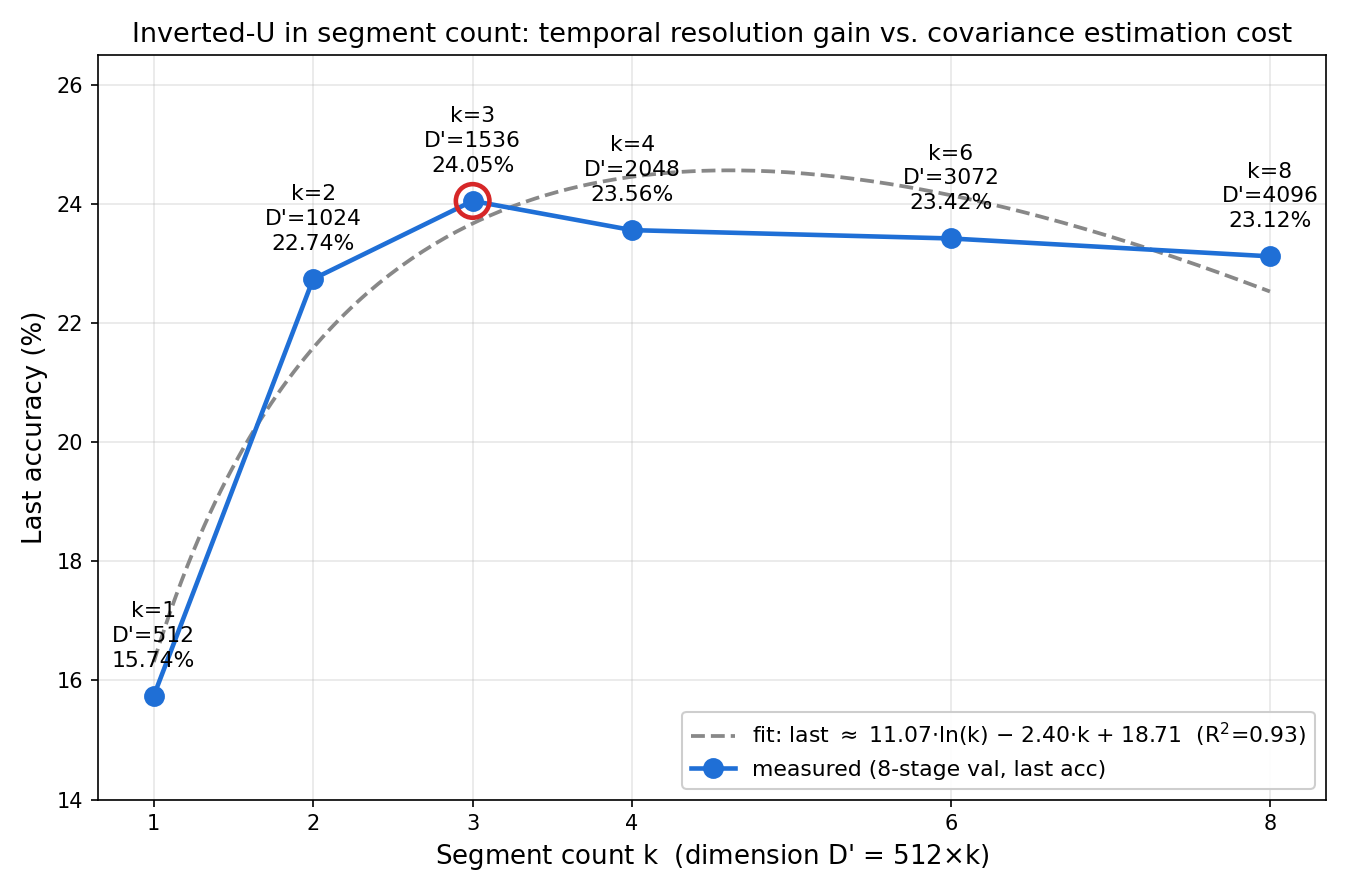
\includegraphics[width=\columnwidth]{assets_segment_count_inverted_u.png}
\caption{Last-session accuracy as a function of segment count $k$ on SSv2
(48-class protocol). A log-linear fit,
$\mathrm{Acc}_{\mathrm{last}}(k) \approx 11.07\ln k - 2.40k + 18.71$
($R^2{=}0.93$), captures the saturating resolution gain (the $\ln k$ term)
against the roughly linear estimation cost (the $k$ term); its extrapolated
maximum near $k^*{\approx}4.6$ is not itself a measured point and should be
read as illustrative rather than confirmed.}
\label{fig:inverted-u}
\end{figure}

\textbf{Overlapping segments do not help.} We also tested widening each
segment so that neighbors overlap, keeping the total output dimension fixed
at $kD$, the standard remedy for hard-boundary artifacts in convolutional
and spectral pooling. On this task, accuracy does not improve and degrades
monotonically as overlap grows (measured in
Section~\ref{sec:experiments}). The reason is mechanistic rather than
incidental: segment pooling helps because each segment owns an exclusive
position in the output, which is what lets the classifier read off order;
overlap makes neighboring segments share frames, so their content converges
toward one another (and, in the limit, toward plain mean pooling) even
though their output positions remain distinct. Widening the window
therefore erodes the very property the method depends on. We report this
as a negative result and do not adopt overlap.

\subsection{Adjacent and Absolute Difference}
\label{sec:method-diff}

\textbf{Two distinct mechanisms.} Segmentation and differencing are mechanistically distinct: a segment
encodes \emph{where} in the window a piece of content sits, while a
difference between adjacent segments encodes \emph{what changed} between
two positions. Treating both as one observation obscures a real dependency:
whether differencing helps depends on whether it is applied at the frame or
the segment level, and, at the segment level, on how many segments already
exist. Figures~\ref{fig:diff-frame-diagram} and~\ref{fig:diff-segment-diagram}
summarize both findings before the numbers do.

\textbf{Frame-level.} Using only the difference between consecutive frames,
with no appearance information at all, performs \emph{worse} than the
mean-pooling baseline: knowing that something moved is not useful without
knowing what moved. Concatenating the mean with the frame-level difference
recovers a substantial gain, and adding the magnitude of that difference
(direction-agnostic) on top of the signed difference improves it further.
The pattern supports a specific design conclusion: adjacent/absolute
difference is not a standalone signal but a secondary one that only helps
once appearance is already represented (quantitative values in
Section~\ref{sec:experiments}).

\begin{figure}[pos=!htb]
\centering
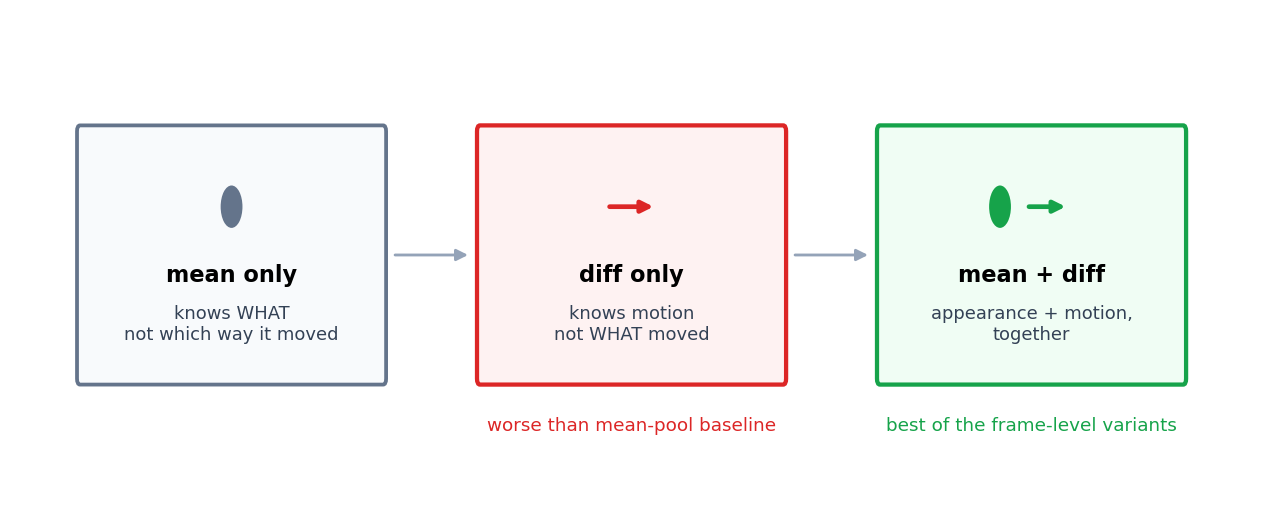
\includegraphics[width=\columnwidth]{assets_diff_diagram_frame.png}
\caption{At the frame level, differencing alone discards appearance and
underperforms the mean-pool baseline, while combining mean and diff is the
best frame-level variant.}
\label{fig:diff-frame-diagram}
\end{figure}

\textbf{Segment-level.} Applying the same idea to the deployed segment
poolings, chunks3 and chunks4, and toggling the difference term on and off
for each, produces a conditional result: at $k{=}3$, adding the difference
term is a consistent win; at $k{=}4$, the effect is far weaker and, by one
of our two accuracy metrics, reverses sign (Section~\ref{sec:experiments}).
The natural reading is that segmentation and differencing partially
duplicate each other as sources of order information: once the window is
already finely segmented ($k{=}4$), there is less temporal information left
for an explicit difference term to add. This direction is corroborated by
an independent measurement (a held-out selection sweep run separately from
the direct $k{=}3$/$k{=}4$ comparison reaches the same conclusion), which
argues against it being an artifact of either single experiment.

\begin{figure*}[width=\textwidth,pos=!t]
\centering
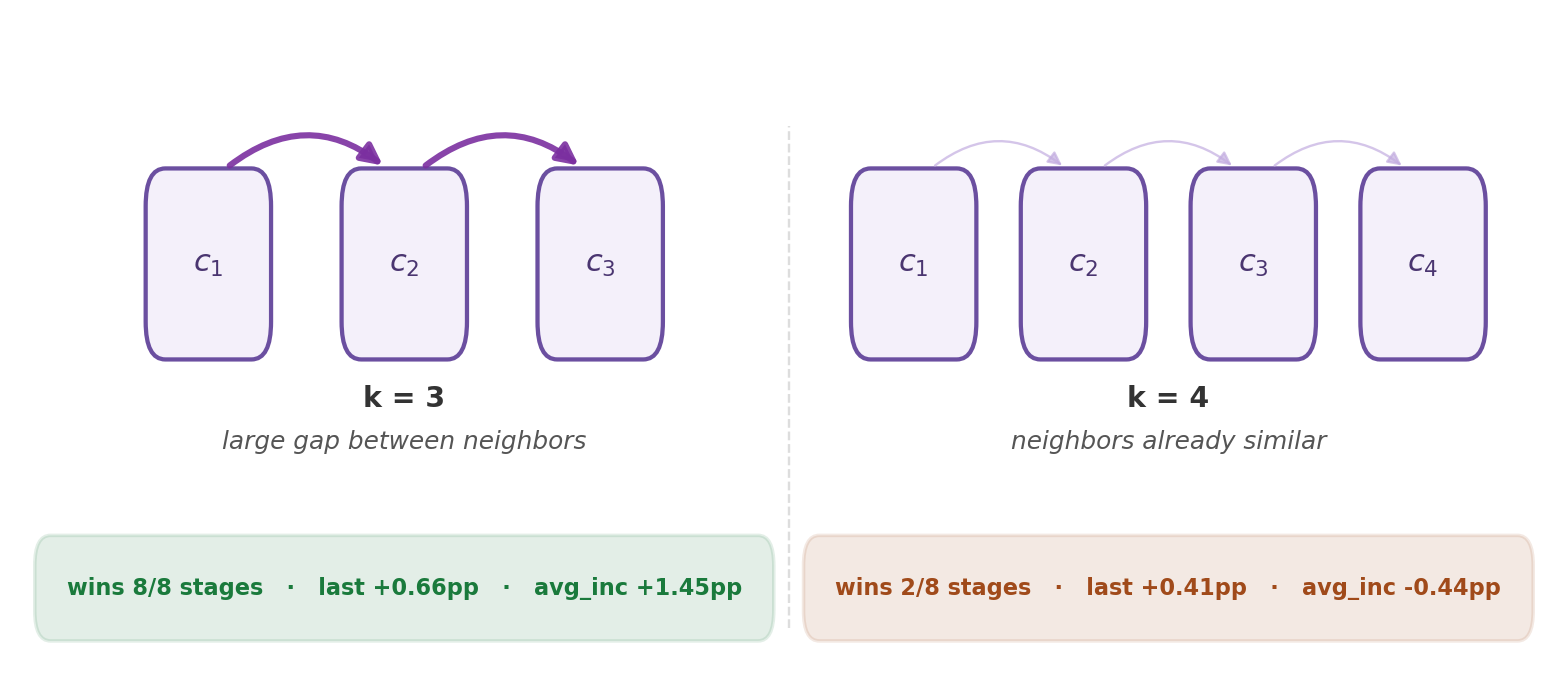
\includegraphics[width=\textwidth]{assets_diff_diagram_segment.png}
\caption{At the segment level, the same adjacent-difference operation
($c_i{-}c_{i-1}$) has opposite value depending on $k$: with $k{=}3$ coarse
segments, neighboring means differ substantially and the diff term wins
every evaluation stage; with $k{=}4$ finer segments, neighboring means are
already close, so the diff term is largely redundant with the segmentation
itself and its benefit becomes inconsistent (arrow thickness is
illustrative of this shrinking gap, not to scale).}
\label{fig:diff-segment-diagram}
\end{figure*}


% =====================================================================
\section{Experiments}
\label{sec:experiments}
% =====================================================================

\subsection{Configuration}

\textbf{Datasets.}
UCF101~\cite{soomro2012ucf101} provides 101 action classes and
13{,}320 clips under official split~1. We follow the TCD~\cite{park2021tcd}
protocol: 51 base classes are learned offline, and the remaining
50 classes are registered incrementally. Table~\ref{tab:ucf101-spec} gives
the exact dataset specification, verified against the original paper.

\begin{table}[pos=!htb]
\centering
\caption{UCF101 specification~\cite{soomro2012ucf101}.}
\label{tab:ucf101-spec}
\small
\begin{tabular}{@{}P{2.8cm}P{4.6cm}@{}}
\toprule
Item & Value \\
\midrule
Classes & 101 \\
Total clips & 13{,}320 \\
Groups per class & 25 \\
Clips per group & 4--7 \\
Total duration & 1{,}600 minutes \\
Clip length range & 1.06\,s -- 71.04\,s \\
Frame rate & 25\,fps \\
Resolution & $320\times240$ \\
Source & YouTube (2012) \\
\bottomrule
\end{tabular}
\end{table}

Something-Something V2~\cite{goyal2017ssv2} (V2 redistribution per
Qualcomm's official release) provides 174 action classes defined
substantially by motion rather than appearance. We use two scales in
parallel: (1) a curated 48-class subset (up to 100 training samples per
class, an 8-stage $\times$ 6-class curriculum) for most ablations and head
comparisons, and (2) the full 174-class set (100 training / 50 validation
samples per class, capped) to reproduce TCD's literal protocol (84 base $+$
either $10{\times}9$ or $5{\times}18$ incremental sessions).
Table~\ref{tab:ssv2-spec} gives the full specification.

\begin{table*}[pos=!t]
\centering
\caption{SSv2 specification.}
\label{tab:ssv2-spec}
\small
\begin{tabular}{@{}P{3.5cm}P{9cm}@{}}
\toprule
Item & Value \\
\midrule
Classes & 174 \\
Total videos & 220{,}847 \\
Train / val / test & 168{,}913 / 24{,}777 / 27{,}157 (unlabeled) \\
Crowd contributors & 5{,}400+ \\
Frame rate & 12\,fps (measured) \\
Codec / container & VP9, WebM \\
Resolution (height) & 240\,px \\
Clip length & $\sim$2--6\,s (literature); measured samples: 3.08\,s (37 frames), 4.67\,s (56 frames) \\
Total download size & 19.4\,GB \\
\bottomrule
\end{tabular}
\end{table*}

\textbf{Feature extraction.} For both datasets, 16 frames are uniformly
sampled per clip (decoded with \texttt{av}) and independently encoded by a
frozen CLIP~\cite{radford2021clip} ViT-B/32 (\texttt{openai/clip-vit-base-patch32}, 512-d),
producing $(16, D)$ raw features per clip. The backbone is fixed for both
datasets; no gradient flows through it at any stage. Pooling is applied to
those raw features at evaluation time, so a pooling variant is a choice of
$\phi$ over fixed inputs, never a re-extraction. Unless a table states
otherwise, headline results use \texttt{chunks3+adjdiff}, and mean pooling
appears only as the baseline it is compared against.

\textbf{Class order and splits.} To avoid results being an artifact of
class order, base/incremental splits are generated from a fixed random seed
permutation, and results reported over multiple seeds average across at
least three class orders.

\textbf{Hyperparameters.} Table~\ref{tab:hyperparams} lists every
hyperparameter used in the experiments below.

\begin{table*}[pos=!t]
\centering
\caption{Hyperparameters.}
\label{tab:hyperparams}
\small
\renewcommand{\arraystretch}{1.15}
\begin{tabular}{@{}P{4.3cm}P{9.5cm}@{}}
\toprule
Component & Value \\
\midrule
Frames per clip & 16 (uniform sampling) \\
Pooling dimension multiplier & mean $1\times$ (512-d) / chunks4 $4\times$ (2048-d) / chunks3+adjdiff $5\times$ (2560-d) \\
FeCAM shrinkage & diagonal $\gamma_1{=}1.0$, off-diagonal $\gamma_2{=}1.0$ (many-shot CIL setting~\cite{goswami2023fecam}) \\
FeCAM few-shot correction & enabled in the deployed configuration; a no-op under balanced samples \\
SLDA shrinkage & isotropic $\lambda{=}0.01$ (diagonal only) \\
SSv2 48-class curriculum & 8 stages $\times$ 6 classes \\
SSv2 174-class (TCD) structure & 84-class base $+$ 90-class incremental ($10{\times}9$ or $5{\times}18$ sessions) \\
UCF101 (TCD) structure & 51-class base $+$ 50-class incremental (5-shot/class exemplar for baselines) \\
Real-time target & 10\,fps ($=$100\,ms/frame), CPU, batch $=$1 (streaming) \\
Timing hardware & Apple M4, 10 cores (4 performance $+$ 6 efficiency), 16\,GB RAM \\
\bottomrule
\end{tabular}
\end{table*}

\textbf{Metrics.} We report two accuracy metrics and two efficiency metrics,
defined in Table~\ref{tab:metrics}. Average incremental accuracy
($\mathrm{Acc}_{\mathrm{avg}}$) is the standard headline metric in CIL
literature since iCaRL~\cite{rebuffi2017icarl}; last-session accuracy ($\mathrm{Acc}_{\mathrm{last}}$)
is the harder, order-invariant number that must be used whenever benchmarks
with different class counts are compared, since $\mathrm{Acc}_{\mathrm{avg}}$
is systematically inflated by early sessions that contain fewer classes.
All reported accuracies use the full class-incremental evaluation (argmax
over every class seen so far, no task/session identity at test time) unless
stated otherwise.

\begin{table*}[pos=!t]
\centering
\caption{Metric definitions.}
\label{tab:metrics}
\small
\begin{tabular}{@{}lP{6.3cm}P{5.7cm}@{}}
\toprule
Metric & Definition & Purpose \\
\midrule
$\mathrm{Acc}_s$ & Val.\ accuracy over all classes seen through session $s$ & One point on the incremental curve \\
$\mathrm{Acc}_{\mathrm{avg}}$ & $\frac{1}{S}\sum_{s=1}^{S}\mathrm{Acc}_s$ & Headline metric (iCaRL convention) \\
$\mathrm{Acc}_{\mathrm{last}}$ & Accuracy at the final session & Hardest, order-invariant; required for cross-benchmark comparison \\
\midrule
FPS & $1000 / (\text{encode}_{\text{1frame}} + \text{pool} + \text{head\_scores})$, ms & Streaming throughput (ring buffer, CPU, batch$=$1) \\
Fit time & Wall-clock to update the head with one session's data & Enrollment cost \\
\bottomrule
\end{tabular}
\end{table*}

\subsection{Results and Discussion}

\textbf{The closed-form/backprop cost gap.} The enrollment-cost claim that
motivates this design (Section~\ref{sec:intro}) is measured directly, not
assumed, on an Apple M4 CPU (10 cores: 4 performance $+$ 6 efficiency,
16\,GB RAM). On our 48-class SSv2 protocol (8 stages, 15 epochs per
stage), fitting the FeCAM head takes 42.4\,ms of wall-clock time, versus
270.0\,s to fine-tune a small GRU baseline (256-unit hidden state, Adam,
learning rate $10^{-4}$, binary cross-entropy loss) with backpropagation
on the same data: a $6{,}400\times$ gap. A hardware-independent accounting
gives the same conclusion: 2.85\,G training FLOPs for FeCAM against
4.64\,T for the GRU baseline, $1{,}628\times$ fewer.

\textbf{Comparison against prior work on UCF101 (TCD protocol).} We verified
protocol agreement directly rather than assuming it: our class order matches
TCD's public repository bit-for-bit across all 101 classes.
Table~\ref{tab:ucf101-compare} places our method next to five methods' own
reported numbers on this exact protocol. We rank second, ahead of TCD by
15.1\,pp, FrameMaker by 11.9\,pp, STSP by 8.9\,pp, and ST-Prompt by
5.2\,pp, and behind only ESSENTIAL, despite using zero exemplars and zero
gradient steps.

\begin{table*}[pos=!t]
\centering
\caption{UCF101, TCD protocol, average incremental accuracy at three
increment granularities (self-reported numbers). Our row uses the
\texttt{chunks3+adjdiff} pooling selected on SSv2
(Section~\ref{sec:method-pooling}), applied here unchanged; the mean-pool
baseline on the identical protocol scores 88.84/88.86/88.84, so
$+1.16$\,pp of our margin comes from the pooling itself.
\texttt{chunks4+adjdiff} scores marginally higher here (90.23), but was
not substituted: the pooling choice was fixed on SSv2 before UCF101 was
evaluated, and substituting it here would be selecting on the test set.
TCD and FrameMaker~\cite{pei2022framemaker} both fine-tune a TSM backbone
throughout training, replaying 5 and an undisclosed number of
exemplars/class respectively; STSP is exemplar-free and is the same method
as Table~\ref{tab:tcd-lineage}, evaluated here on UCF101 instead of SSv2;
ST-Prompt~\cite{pei2023stprompt} keeps CLIP frozen and instead trains
space-time prompts via backpropagation; ESSENTIAL keeps CLIP frozen but
trains a temporal encoder and classifier via backpropagation
(24$\times$RTX~3090); we use frozen CLIP with zero exemplars and zero
gradient steps at any point. Our $\mathrm{Acc}_{\mathrm{avg}}$ here
averages over all $S$ sessions including the last (Table~\ref{tab:metrics});
TCD/FrameMaker/ST-Prompt's own convention (confirmed against the CSTA
paper) instead averages over the first $S{-}1$ sessions only, which would
give 89.12/89.00/88.90 for our method, a 0.06--0.28\,pp difference that
does not affect the ranking.}
\label{tab:ucf101-compare}
\small
\begin{tabular}{@{}lccc@{}}
\toprule
Method & $10\times5$ & $5\times10$ & $2\times25$ \\
\midrule
TCD~\cite{park2021tcd} (ICCV'21) & 74.89 & 73.43 & 72.19 \\
FrameMaker~\cite{pei2022framemaker} (NeurIPS'22) & 78.13 & 76.38 & 75.77 \\
STSP~\cite{cheng2024stsp} (ECCV'24) & 81.15 & 82.84 & 79.25 \\
ST-Prompt~\cite{pei2023stprompt} (ICCV'23) & 84.80 & 85.50 & 85.70 \\
\textbf{Ours (frozen CLIP + FeCAM + \texttt{chunks3+adjdiff})} & \textbf{90.00} & \textbf{89.99} & \textbf{89.97} \\
ESSENTIAL~\cite{lee2025essential} (ICCV'25) & 95.1 & 93.9 & 93.3 \\
\bottomrule
\end{tabular}
\end{table*}

\textbf{Invariance to increment granularity.} Table~\ref{tab:invariance}
shows a structural property rather than a coincidence. As increments are
split into smaller and smaller groups, every other method's accuracy
moves, mostly downward (TCD $-2.70$\,pp, FrameMaker $-2.36$\,pp, ESSENTIAL
$-1.80$\,pp), sometimes non-monotonically (STSP rises at the middle
granularity before falling, net $-1.90$\,pp) or even upward (ST-Prompt,
$+0.90$\,pp); ours moves by $-0.03$\,pp, an order of magnitude less than
any of them. The residual 0.03 is not model drift but an artifact of the
metric: $\mathrm{Acc}_{\mathrm{avg}}$ averages over the evaluation points a
schedule happens to define, and the three schedules define 6, 11, and 26 of
them. The quantity that is invariant by construction is
$\mathrm{Acc}_{\mathrm{last}}$, accuracy once all 101 classes are enrolled,
and it is bit-identical at 88.61 under all three schedules. Both follow
from the closed-form update rule: a running mean and covariance converge to
the same statistics regardless of the order or grouping in which the
underlying samples arrive, a guarantee no gradient-trained method in this
comparison shares.
The practical implication is not an accuracy advantage but a
deployment-reliability one: in an environment where the number and timing
of newly arriving classes is not known in advance, this property
guarantees that performance cannot be shifted by an unfavorable enrollment
schedule in either direction.

\begin{table}[pos=!htb]
\centering
\caption{Change in accuracy from the coarsest to the finest increment
granularity on UCF101 (same methods as Table~\ref{tab:ucf101-compare}).
$^\dagger$STSP is non-monotonic across the three granularities
(81.15 $\to$ 82.84 $\to$ 79.25); the figure shown uses only the two
endpoints.}
\label{tab:invariance}
\small
\begin{tabular}{@{}lc@{}}
\toprule
Method & $10\times5 \to 2\times25$ \\
\midrule
TCD & $74.89 \to 72.19$ ($-2.70$) \\
FrameMaker & $78.13 \to 75.77$ ($-2.36$) \\
STSP$^\dagger$ & $81.15 \to 79.25$ ($-1.90$) \\
ST-Prompt & $84.80 \to 85.70$ ($+0.90$) \\
ESSENTIAL & $95.1 \to 93.3$ ($-1.80$) \\
\textbf{Ours} & $90.00 \to 89.97$ (\textbf{$-0.03$}) \\
\bottomrule
\end{tabular}
\end{table}

\textbf{Ablation: segment count.} Figure~\ref{fig:inverted-u} shows that
accuracy peaks at 3--4 segments and declines beyond that point, confirming
that finer segmentation is not simply better: the temporal-resolution /
covariance-estimability trade-off from Section~\ref{sec:method-pooling}
is real and measurable.

\textbf{Ablation: adjacent/absolute difference.} Table~\ref{tab:diff-frame}
isolates the frame-level effect of differencing before segmentation is
introduced: differencing alone (no appearance) underperforms the mean-pool
baseline, while appending the signed difference, and then its magnitude,
improves steadily.

\begin{table}[pos=!htb]
\centering
\caption{Frame-level diff ablation (mean 512-d baseline). O marks an
included component.}
\label{tab:diff-frame}
\small
\begin{tabular}{@{}cccccc@{}}
\toprule
mean & std & diff & $|$diff$|$ & dim. & $\mathrm{Acc}_{\mathrm{avg}}$ / $\mathrm{Acc}_{\mathrm{last}}$ \\
\midrule
O & & & & 512 & 24.19 / 15.74 \\
O & O & & & 1024 & 24.69 / 16.78 \\
 & & O & & 512 & 22.65 / 13.12 \\
O & & O & & 1024 & 30.50 / 20.69 \\
O & & O & O & 1536 & 30.82 / 21.50 \\
\bottomrule
\end{tabular}
\end{table}

Table~\ref{tab:diff-segment} isolates the same question at the segment
level, for the two deployment-candidate poolings. At $k{=}3$, adding the
difference term wins in all 8 of 8 evaluation stages; at $k{=}4$, it wins
in only stages 6 and 8, losing the remaining six (by
$-1.83$ to $-0.05$\,pp), which is why the $k{=}4$ effect reverses sign
under $\mathrm{Acc}_{\mathrm{avg}}$ even though it stays (barely) positive
under $\mathrm{Acc}_{\mathrm{last}}$. \texttt{chunks4+adjdiff} is
simultaneously the most expensive of the four combinations (dim.\ 3584, fit
10.4\,s) and the least certain to help, which is grounds to exclude it from
deployment.

\begin{table*}[pos=!t]
\centering
\caption{Segment-level diff ablation on the deployment candidates.}
\label{tab:diff-segment}
\small
\begin{tabular}{@{}lccccc@{}}
\toprule
& no diff (dim.) & $+$diff (dim.) & $\Delta\,\mathrm{Acc}_{\mathrm{last}}$ & $\Delta\,\mathrm{Acc}_{\mathrm{avg}}$ & stages won (of 8) \\
\midrule
$k{=}3$ & 24.05 (1536) & \textbf{24.71} (2560) & \textbf{+0.66} & +1.45 & \textbf{S1--S8 (8/8)} \\
$k{=}4$ & 23.56 (2048) & 23.97 (3584) & $+0.41$ & \textbf{$-0.44$} & S6, S8 only (2/8) \\
\bottomrule
\end{tabular}
\end{table*}

\textbf{Scaling to the standard 174-class split.} The ablations above use
our 48-class curriculum; Table~\ref{tab:tcd-lineage} tabulates prior work
on SSv2's actual 174-class TCD split without our method appearing on it.
Table~\ref{tab:ssv2-174} closes that gap, holding the FeCAM head fixed and
sweeping the same pooling variants. Order-preserving pooling beats mean
pooling by a wide margin at this scale too, and \texttt{chunks3+adjdiff}
again leads every variant tested, $+6.77$\,pp $\mathrm{Acc}_{\mathrm{last}}$
and $+6.74$\,pp $\mathrm{Acc}_{\mathrm{avg}}$ over mean pooling. One
ranking does not repeat: without differencing, \texttt{chunks4} edges
\texttt{chunks3} here (by $0.24$\,pp $\mathrm{Acc}_{\mathrm{last}}$), the
reverse of the 48-class order (\texttt{chunks3} ahead by $0.49$\,pp,
Table~\ref{tab:diff-segment}'s no-diff column); both margins sit inside
this experiment's seed-to-seed noise ($\pm0.18$--$0.20$\,pp on
$\mathrm{Acc}_{\mathrm{avg}}$). Once the difference term is added the
ranking is unambiguous at both scales. $\mathrm{Acc}_{\mathrm{last}}$ is
again exactly invariant here: identical to the digits shown across all
three seeds and between the $10{\times}9$/$5{\times}18$ schedules, the same
structural property Table~\ref{tab:invariance} established for UCF101, now
confirmed on a second dataset at $3.6\times$ the class count. Absolute
accuracy stays well below the backprop-trained methods in
Table~\ref{tab:tcd-lineage} (18.50 here against STSP's 70.87, the
strongest entry in that table); Section~\ref{sec:related} already
explains why, since those methods adapt their backbone to SSv2 motion
during training and ours never does. The trade-off is explicit, not
incidental: this paper recovers the order signal mean pooling discards,
not the larger gap that comes from training on SSv2 motion at all.

\begin{table*}[pos=!t]
\centering
\caption{Order-preserving pooling on SSv2's standard 174-class TCD split
(84 base $+$ 90 incremental classes), FeCAM head, mean $\pm$ std over 3
seeds. TCD's own 84-class base set is not published, so seeds vary a
random partition rather than reproducing its literal split (structure and
scale only, not the exact class assignment).
$\mathrm{Acc}_{\mathrm{last}}$ does not vary across seeds or between the
$10{\times}9$/$5{\times}18$ schedules to the precision shown.}
\label{tab:ssv2-174}
\small
\begin{tabular}{@{}lcccc@{}}
\toprule
Pooling & $D$ & $\mathrm{Acc}_{\mathrm{last}}$ & $\mathrm{Acc}_{\mathrm{avg}}$ ($10{\times}9$) & $\mathrm{Acc}_{\mathrm{avg}}$ ($5{\times}18$) \\
\midrule
mean & 512 & 11.74 & 14.42 $\pm$ 0.19 & 14.39 $\pm$ 0.20 \\
chunks3 & 1536 & 17.55 & 20.46 $\pm$ 0.19 & 20.42 $\pm$ 0.19 \\
chunks4 & 2048 & 17.79 & 20.81 $\pm$ 0.19 & 20.76 $\pm$ 0.18 \\
\textbf{chunks3+adjdiff} & 2560 & \textbf{18.50} & \textbf{21.17 $\pm$ 0.14} & \textbf{21.12 $\pm$ 0.16} \\
chunks4+adjdiff & 3584 & 18.15 & 20.98 $\pm$ 0.29 & 20.95 $\pm$ 0.28 \\
\bottomrule
\end{tabular}
\end{table*}

\textbf{Ablation: head choice.} Table~\ref{tab:head-ladder} confirms the
NCM $\to$ SLDA $\to$ FeCAM ladder from Section~\ref{sec:method-fecam}
empirically: accuracy rises monotonically with how much covariance
structure the head uses, at the cost of higher (but still sub-second) fit
time.

\begin{table}[pos=!htb]
\centering
\caption{Head comparison on SSv2 (48-class protocol).}
\label{tab:head-ladder}
\small
\begin{tabular}{@{}lccc@{}}
\toprule
Head & $\mathrm{Acc}_{\mathrm{avg}}$ & $\mathrm{Acc}_{\mathrm{last}}$ & Fit time (s) \\
\midrule
NCM & 20.89 & 12.38 & 0.08 \\
SLDA & 22.77 & 14.14 & 0.13 \\
\textbf{FeCAM} & \textbf{24.19} & \textbf{15.74} & 0.40 \\
\bottomrule
\end{tabular}
\end{table}

\textbf{Finding the best deployable combination.} Finally,
Figure~\ref{fig:combo-sweep} places all nine pooling$\times$head
combinations on a single accuracy-versus-throughput plane on CLIP B/32.
Every combination clears the 10\,fps real-time budget by a wide margin
(39.4--41.6\,fps), so throughput does not constrain the choice within this
scope: the decision reduces to accuracy alone, and FeCAM dominates NCM and
SLDA under every pooling variant tested.

\begin{figure}[pos=!htb]
\centering
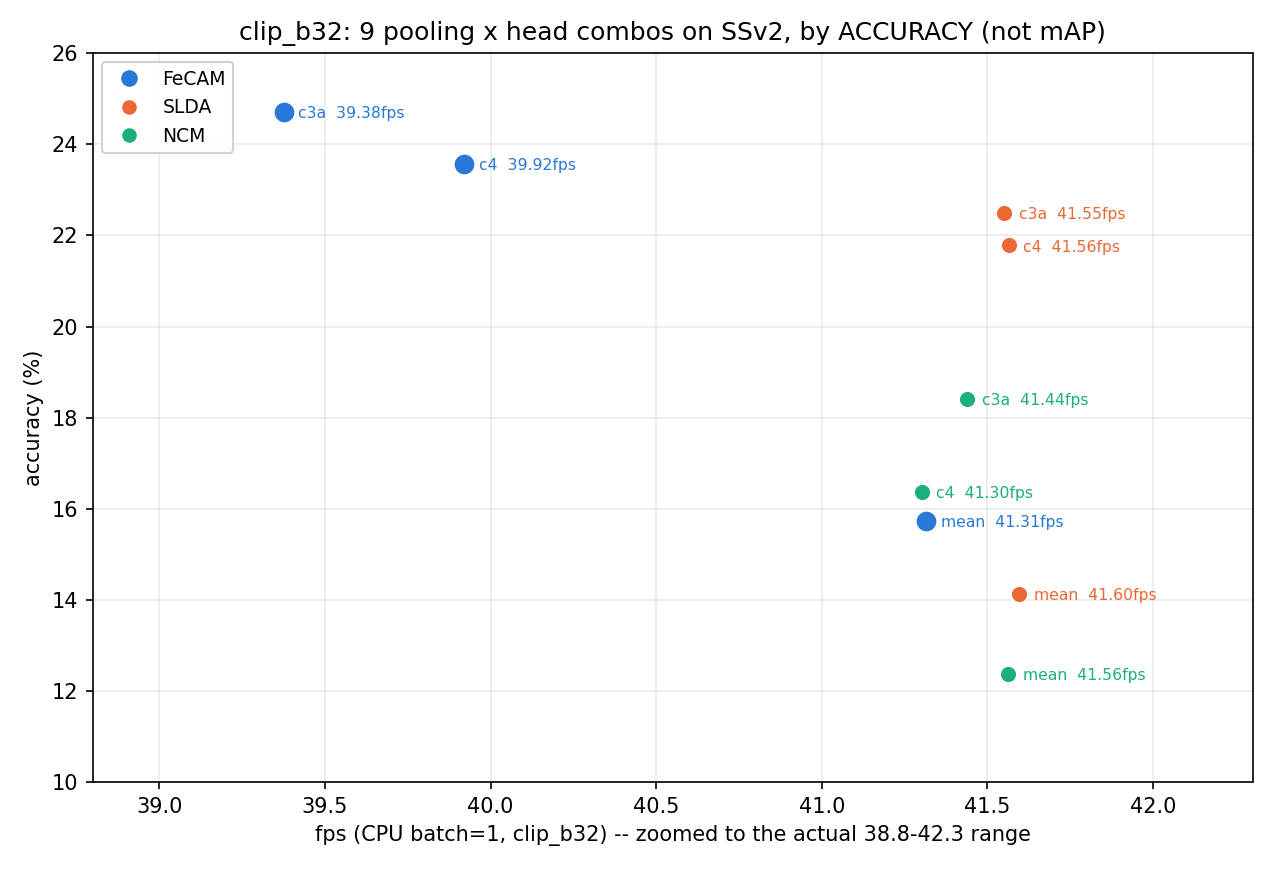
\includegraphics[width=\columnwidth]{assets_ap_fps_sweep_accuracy.png}
\caption{Accuracy vs.\ throughput for nine pooling$\times$head combinations
on SSv2 (CLIP B/32, CPU, batch$=$1). All nine combinations sit well inside
the 10\,fps budget; FeCAM leads at every pooling setting.}
\label{fig:combo-sweep}
\end{figure}


% =====================================================================
\section{Conclusion}
\label{sec:conclusion}
% =====================================================================

\textbf{Summary.} This paper asked whether video class-incremental learning
can be made to work without a GPU, without exemplar replay, and without a
single gradient step after deployment. Starting from the recipe that
already works for image CIL (a frozen backbone plus a closed-form
covariance head), we identified the one component that recipe is missing
for video: a way to preserve the order of frames instead of averaging it
away. Order-preserving temporal pooling closes that gap by splitting each
window into $k$ contiguous segments and concatenating their means, so that
early-then-late and late-then-early occupy different coordinates instead of
the same one. The pooling function and the FeCAM head together add zero
learnable parameters and zero gradient steps to the frozen-backbone
pipeline.

\textbf{What the ablations show.} The gain is front-loaded and mechanistic
rather than incremental. Splitting a window into just two segments already
recovers 78\% of the total improvement over mean pooling, and accuracy
traces an inverted U in segment count that peaks at $k{=}3$--$4$ on our
data scale rather than rising monotonically, which rules out ``more
segments is always better'' as an explanation. Widening segments so that
neighbors overlap, the standard fix for boundary artifacts elsewhere,
instead degrades accuracy monotonically here: overlap is precisely what
erodes the property the method depends on. Adjacent-frame differencing
helps once appearance is already represented but hurts alone, and at the
segment level its value is conditional: a consistent win at $k{=}3$ (8 of 8
stages) and a marginal, sign-reversing one at $k{=}4$ (2 of 8), evidence
that segmentation and differencing partially duplicate each other as
sources of order information rather than stacking for free. The same
ranking, \texttt{chunks3+adjdiff} ahead of every other pooling tested,
reappears on SSv2's standard 174-class split at $3.6\times$ the class
count (Table~\ref{tab:ssv2-174}), together with the same exact
last-session invariance to session grouping established for UCF101 in
Table~\ref{tab:invariance}.

\textbf{Where this leaves us against prior work.} On UCF101 under the TCD
protocol, the method ranks second behind only ESSENTIAL, ahead of TCD,
FrameMaker, STSP, and ST-Prompt, despite using zero exemplars and zero
gradient steps where every other entry in that table uses at least one. It
also has a property none of them share: accuracy is invariant to how
coarsely or finely the incremental sessions are grouped. Last-session
accuracy is bit-identical across the $10\times5$, $5\times10$, and
$2\times25$ schedules, and average incremental accuracy moves by
$-0.03$\,pp against $-2.70$\,pp for TCD and $-1.80$\,pp for ESSENTIAL. That invariance is not a
tuned result but a direct consequence of closed-form updates being
independent of arrival order, and it matters operationally more than as a
leaderboard number: a deployed system cannot always control how classes
arrive, and this property guarantees no enrollment schedule can make it
worse. All nine pooling$\times$head combinations tested clear the 10\,fps
real-time budget with room to spare (39.4--41.6\,fps on CPU), so this
ranking is not purchased at the cost of throughput.

\textbf{Limitations.} Two scope choices should be stated plainly. First,
Table~\ref{tab:ssv2-174} reports our own numbers on SSv2's standard
174-class split, but TCD's own 84-class base set is not published, so the
base/incremental partition there is random per seed rather than a
reproduction of the literal split; the comparison matches TCD's structure
and scale, not necessarily its exact class assignment. Second, every main
result in this paper uses frozen CLIP ViT-B/32; a supplementary check on a
second CLIP-family checkpoint (OpenCLIP~\cite{ilharco2021openclip} ViT-L/14 trained on
LAION-2B~\cite{schuhmann2022laion5b}, \texttt{laion/CLIP-ViT-L-14-laion2B-s32B-b82K}; different
training data and width) reproduces the same pooling ranking and a comparable gain over
mean pooling ($+8.7$--$9.7$\,pp across pooling variants, versus
$+7.8$--$9.0$\,pp on CLIP B/32), which rules out an artifact of that one
checkpoint specifically. Both backbones tested, however, share the same
contrastive image-text pretraining with no temporal signal of any kind, so
whether the gain persists on a backbone from a different pretraining
paradigm, or one whose frame features already carry some temporal
information, remains untested; the accuracy ceiling on motion-heavy
classes likewise remains set by what a backbone never trained on SSv2 can
represent, a ceiling this paper does not attempt to raise.

\textbf{Future work.} Two directions follow from the deployment scenario
in Section~\ref{sec:intro}. One is empirical: measuring few-shot live
enrollment directly, how many example clips a new class needs before
FeCAM's mean and covariance estimate stabilize, rather than assuming the
sample counts used throughout this paper. The other is architectural:
testing whether order-preserving pooling composes with other frozen
backbones and modalities, since nothing in its construction is
CLIP-specific. Both keep the constraint this paper set out to satisfy:
whatever is added must still run, and still update, on the device that
shipped it.

% ---- Back matter required at submission (Neurocomputing / Elsevier) ----
\printcredits

\section*{Declaration of competing interest}
The author declares that they have no known competing financial interests
or personal relationships that could have appeared to influence the work
reported in this paper.

\section*{Data availability}
All experiments use publicly available datasets: UCF101~\cite{soomro2012ucf101}
and Something-Something V2~\cite{goyal2017ssv2}. Frame features were
extracted with publicly released frozen encoders
(\texttt{openai/clip-vit-base-patch32} and
\texttt{laion/CLIP-ViT-L-14-laion2B-s32B-b82K}). The code and extracted
features used in this study are available from the corresponding author
upon reasonable request.

\section*{Declaration of generative AI and AI-assisted technologies in the manuscript preparation process}
During the preparation of this work the author used Claude (Anthropic) in
order to draft and revise text for clarity and structure, and to format
the manuscript. After using this tool, the author reviewed and edited the
content as needed and takes full responsibility for the content of the
published article.

\bibliographystyle{elsarticle-num}
\bibliography{references}

\end{document}
